\ifdefined\inMainDoc\else
\documentclass[12pt,a4paper]{article}
% ================================================================
%  PRÉAMBULE COMMUN - ANNALES CORRIGÉES
%  Université de Kara - FaST - Licence Fondamentale MPC
%  Design optimisé impression noir et blanc
% ================================================================

% -- ENCODAGE & LANGUE --
\usepackage[utf8]{inputenc}
\usepackage[T1]{fontenc}
\usepackage[french]{babel}
\usepackage{lmodern}
\usepackage{microtype}

% -- MISE EN PAGE --
\usepackage[a4paper, top=2.8cm, bottom=2.5cm, left=2.5cm, right=2.5cm, headheight=14pt]{geometry}
\usepackage{setspace}
\setstretch{1.2}
\usepackage{parskip}
\setlength{\parindent}{1.2em}
\setlength{\parskip}{4pt}

% -- MATHS --
\usepackage{amsmath, amssymb, mathtools, amsthm}
\usepackage{mathrsfs}
\usepackage{dsfont}
\usepackage{bm}
\usepackage{cancel}
\usepackage{textcomp}
% Définition de \oiint (intégrale de surface fermée) sans package supplémentaire
\newcommand{\oiint}{\mathop{\iint\!\!\!\!\!\!\!\bigcirc}\limits}

% -- PHYSIQUE & CHIMIE --
\usepackage{physics}
\usepackage{siunitx}
% Lorsque physics est chargé, siunitx omet \qty. On le restaure ici :
\AtBeginDocument{\RenewCommandCopy\qty\SI}
\sisetup{locale = FR, detect-all, output-decimal-marker={,}}
% Commande de substitution pour les unités posant problème avec pdflatex
% (ohm, degreeCelsius, micro, angstrom, percent utilisent des caractères non-ASCII)
\newcommand{\qtyohm}[1]{\ensuremath{\num{#1}\,\Omega}}
\newcommand{\qtydegc}[1]{\ensuremath{\num{#1}\,{}^\circ\text{C}}}
\newcommand{\qtyangstrom}[1]{\ensuremath{\num{#1}\,\text{\AA}}}
\newcommand{\qtypercent}[1]{\ensuremath{\num{#1}\,\%}}
\newcommand{\qtyum}[1]{\ensuremath{\num{#1}\,\mu\text{m}}}
\usepackage[version=4]{mhchem}

% -- GRAPHISMES --
\usepackage{graphicx}
\usepackage{float}
\usepackage{caption}
\usepackage{subcaption}
\usepackage{wrapfig}
\usepackage{tikz}
\usetikzlibrary{calc, arrows.meta, patterns, shapes.geometric}
\usepackage{pgfplots}
\pgfplotsset{compat=1.18}

% -- TABLEAUX --
\usepackage{booktabs}
\usepackage{array}
\usepackage{tabularx}
\usepackage{multirow}

% -- LISTES --
\usepackage{enumitem}
\setlist[enumerate]{topsep=3pt, itemsep=2pt, parsep=0pt}
\setlist[itemize]{topsep=3pt, itemsep=2pt, parsep=0pt, label={.}}

% -- BOÎTES (noir et blanc) --
\usepackage{mdframed}
\usepackage{tcolorbox}
\tcbuselibrary{skins, breakable, theorems}

% Boîte EXERCICE : encadré avec filet épais, fond blanc
\newmdenv[
  linewidth=1.2pt,
  linecolor=black,
  roundcorner=3pt,
  skipabove=10pt,
  skipbelow=6pt,
  innertopmargin=8pt,
  innerbottommargin=8pt,
  innerleftmargin=10pt,
  innerrightmargin=10pt,
  backgroundcolor=white,
  frametitle={\bfseries\small Exercice},
  frametitlealignment=\raggedright,
  frametitleaboveskip=4pt,
  frametitlebelowskip=4pt,
]{boiteexercice}

% Boîte CORRIGÉ : fond gris très clair + filet fin
\newmdenv[
  linewidth=0.6pt,
  linecolor=black,
  leftline=true,
  rightline=false,
  topline=false,
  bottomline=false,
  linecolor=black,
  innerleftmargin=12pt,
  innerrightmargin=8pt,
  innertopmargin=6pt,
  innerbottommargin=6pt,
  backgroundcolor=gray!8,
  skipabove=4pt,
  skipbelow=8pt,
]{boitecorrige}

% Boîte RÉSUMÉ DE COURS : double encadré
\newmdenv[
  linewidth=0.8pt,
  linecolor=black,
  roundcorner=2pt,
  backgroundcolor=gray!12,
  innertopmargin=10pt,
  innerbottommargin=10pt,
  innerleftmargin=12pt,
  innerrightmargin=12pt,
  skipabove=12pt,
  skipbelow=8pt,
]{boiteresume}

% Boîte ATTENTION/REMARQUE : barre gauche épaisse
\newmdenv[
  leftline=true,
  rightline=false,
  topline=false,
  bottomline=false,
  linewidth=3pt,
  linecolor=black,
  backgroundcolor=gray!5,
  innerleftmargin=12pt,
  innerrightmargin=8pt,
  innertopmargin=5pt,
  innerbottommargin=5pt,
  skipabove=6pt,
  skipbelow=6pt,
]{boiteremarque}

% -- DIFFICULTÉ DES EXERCICES --
\newcommand{\facile}{$\star$}
\newcommand{\moyen}{$\star\!\star$}
\newcommand{\difficile}{$\star\!\star\!\star$}
\newcommand{\niveau}[1]{\hfill\textbf{#1}\hspace{2pt}}

% -- EN-TÊTES ET PIEDS DE PAGE --
\usepackage{fancyhdr}
\pagestyle{fancy}
\fancyhf{}
\renewcommand{\headrulewidth}{0.5pt}
\renewcommand{\footrulewidth}{0.3pt}

% -- HYPERLIENS --
\usepackage[hidelinks]{hyperref}
\hypersetup{
    colorlinks=false,
    pdftitle={Annale Corrigée - Licence MPC - Université de Kara}
}

% -- TITRES --
\usepackage{titlesec}
\titleformat{\section}{\Large\bfseries}{\thesection.}{0.8em}{}[\vspace{2pt}\hrule\vspace{4pt}]
\titleformat{\subsection}{\large\bfseries}{\thesubsection.}{0.7em}{}
\titleformat{\subsubsection}{\normalsize\bfseries}{\thesubsubsection.}{0.6em}{}

% -- THÉORÈMES --
\theoremstyle{definition}
\newtheorem{defn}{Définition}[section]
\newtheorem{prop}{Propriété}[section]
\newtheorem{thm}{Théorème}[section]
\newtheorem{corol}{Corollaire}[section]
\newtheorem{exemple}{Exemple}[section]

% -- COMMANDES MATHÉMATIQUES UTILES --
\newcommand{\vect}[1]{\overrightarrow{#1}}
\newcommand{\R}{\mathbb{R}}
\newcommand{\N}{\mathbb{N}}
\newcommand{\Z}{\mathbb{Z}}
\newcommand{\C}{\mathbb{C}}
\renewcommand{\d}{\mathrm{d}}
\newcommand{\deriv}[2]{\dfrac{\d #1}{\d #2}}
\newcommand{\dpart}[2]{\dfrac{\partial #1}{\partial #2}}
\newcommand{\rot}{\overrightarrow{\mathrm{rot}}\,}
\renewcommand{\div}{\mathrm{div}\,}
\renewcommand{\grad}{\overrightarrow{\mathrm{grad}}\,}
\newcommand{\e}{\mathrm{e}}
\newcommand{\ii}{\mathrm{i}}
\renewcommand{\Tr}{\mathrm{Tr}}

% Numérotation des équations par section
\numberwithin{equation}{section}

% -- RÉSULTATS ENCADRÉS --
\newcommand{\res}[1]{\[\boxed{#1}\]}

% -- REMARQUE INLINE --
\newcommand{\rmq}[1]{\begin{boiteremarque}\textbf{Remarque.} #1\end{boiteremarque}}

% -- MISE EN VALEUR DU RÉSULTAT FINAL --
\newcommand{\reponse}[1]{%
  \begin{center}
    \fbox{\begin{minipage}{0.92\textwidth}\centering #1\end{minipage}}
  \end{center}%
}


\lhead{\small\textit{Électrocinétique - Licence 1}}
\rhead{\small\textit{FaST, Université de Kara}}
\cfoot{\thepage}

\begin{document}
\fi

\begin{center}
  {\LARGE\bfseries ÉLECTROCINÉTIQUE ET RÉGIME VARIABLE}\\[0.3cm]
  {\normalsize Licence 1 - Mathématiques, Physique et Chimie}\\[0.1cm]
  \rule{0.7\textwidth}{0.8pt}
\end{center}

\vspace{0.3cm}

% ================================================================
\section*{Résumé du cours}
% ================================================================

\begin{boiteresume}

\textbf{1. Lois fondamentales.}
\begin{itemize}[nosep]
  \item \textbf{Loi des n\oe{}uds (Kirchhoff courant)} : la somme algébrique des courants entrant en un n\oe{}ud est nulle : $\sum I_k = 0$.
  \item \textbf{Loi des mailles (Kirchhoff tension)} : la somme algébrique des tensions le long d'une maille fermée est nulle : $\sum U_k = 0$.
  \item \textbf{Loi d'Ohm} (convention récepteur) : $U = RI$.
\end{itemize}

\textbf{2. Associations de résistances.}
\begin{itemize}[nosep]
  \item En série : $R_{eq} = R_1 + R_2 + \cdots$
  \item En parallèle : $\dfrac{1}{R_{eq}} = \dfrac{1}{R_1} + \dfrac{1}{R_2} + \cdots$
\end{itemize}

\textbf{3. Diviseur de tension et diviseur de courant.}
\[
U_{R_2} = \frac{R_2}{R_1 + R_2}\,E \qquad I_{R_2} = \frac{G_2}{G_1 + G_2}\,I = \frac{R_1}{R_1 + R_2}\,I
\]
(avec $G_k = 1/R_k$ la conductance).

\textbf{4. Théorèmes de Thévenin et Norton.}
\begin{itemize}[nosep]
  \item \textbf{Thévenin} : tout circuit linéaire vu de deux bornes A, B est équivalent à une source de tension $E_{th}$ (tension à vide entre A et B) en série avec $R_{th}$ (résistance vue des bornes avec les sources éteintes).
  \item \textbf{Norton} : équivalent de Thévenin $\to$ Norton via $I_N = E_{th}/R_{th}$, résistance identique $R_{th}$.
\end{itemize}

\textbf{5. Théorème de Millman.}
Pour $n$ branches en parallèle entre les n\oe{}uds A et B :
\[
U_{AB} = \frac{\displaystyle\sum_{k=1}^{n} \frac{\varepsilon_k}{R_k}}{\displaystyle\sum_{k=1}^{n} \frac{1}{R_k}}
\]
où $\varepsilon_k$ est la f.é.m. de la $k$-ième branche (comptée positivement si elle pousse de B vers A).

\textbf{6. Puissance transmise à une charge.} La puissance maximale est transmise à une charge $R_L$ lorsque $R_L = R_{th}$ (condition d'adaptation d'impédance) :
\[
P_{\max} = \frac{E_{th}^2}{4R_{th}}
\]

\end{boiteresume}

\newpage

% ================================================================
\section{Circuits résistifs et théorèmes}
% ================================================================

\subsection*{Exercice 1 - Réseau à deux mailles \niveau{\moyen}}

\begin{boiteexercice}
\begin{minipage}{0.6\textwidth}
Déterminer, pour le circuit ci-contre, l'intensité $i$ traversant $R_2$ et la tension $u$ aux bornes de $R_3$ :
\begin{enumerate}
  \item en faisant des associations de résistances et en appliquant le diviseur de tension ;
  \item en faisant une transformation Thévenin $\to$ Norton et en appliquant le diviseur de courant.
  \item Application numérique : $E = \qty{6}{V}$, $R_1 = \qtyohm{100}$, $R_2 = R_3 = R_4 = \qtyohm{50}$.
\end{enumerate}
\end{minipage}
\hfill
\begin{minipage}{0.35\textwidth}
\centering
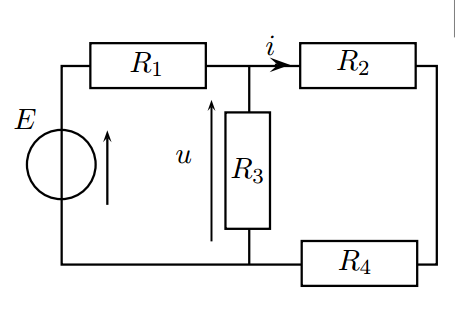
\includegraphics[width=\textwidth]{images/el2.png}
\end{minipage}
\end{boiteexercice}

\begin{boitecorrige}
\textbf{1. Méthode par associations.}

$R_2$ et $R_4$ sont en série : $R_5 = R_2 + R_4$.

$R_3$ et $R_5$ sont en parallèle :
\[
R_6 = \frac{R_3 R_5}{R_3 + R_5}
\]
$R_1$ et $R_6$ sont en série, soumis à $E$. La tension $u = U_{AB}$ est donnée par le diviseur de tension :
\[
\boxed{u = U_{AB} = \frac{R_3(R_2+R_4)}{R_1 R_3 + (R_1+R_3)(R_2+R_4)}\,E}
\]
Le courant dans $R_5$ (donc dans $R_2$) :
\[
\boxed{i = \frac{u}{R_5} = \frac{R_3\,E}{R_1 R_3 + (R_1+R_3)(R_2+R_4)}}
\]

\begin{boiteremarque}
$i$ n'apparaît plus dans le schéma simplifié final. Il faut revenir au schéma intermédiaire (avant la mise en parallèle de $R_3$ et $R_5$) pour l'exprimer.
\end{boiteremarque}

\textbf{2. Transformation Thévenin $\to$ Norton.}

Entre les n\oe{}uds A et B, on a un générateur de Thévenin ($E$, $R_1$). Transformation en Norton : $\eta = E/R_1$, résistance équivalente $R_0 = R_1 R_3/(R_1 + R_3)$ (après mise en parallèle de $R_1$ et $R_3$). Le diviseur de courant donne le même résultat qu'à la question 1.

\textbf{3. Application numérique :} $R_5 = 100\,\Omega$, $R_6 = R_3 R_5/(R_3+R_5) = 50\times100/150 \approx 33{,}3\,\Omega$.
\[
u = \frac{33{,}3}{100+33{,}3}\times 6 \approx \qty{1.5}{V} \qquad i = \frac{1{,}5}{100} = \qty{15}{mA}
\]
\end{boitecorrige}

\begin{center}
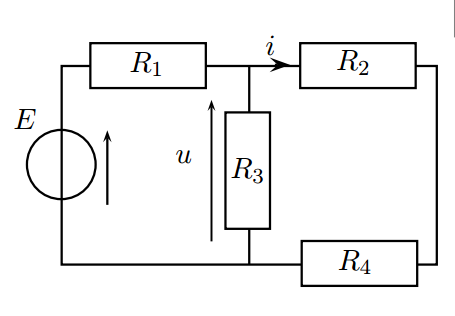
\includegraphics[width=0.6\textwidth]{images/electrocinetique/elec-001-000.png}
\captionof{figure}{\small Schéma du réseau à deux mailles avec courants et tensions.}
\end{center}
\begin{center}

\includegraphics[width=0.6\textwidth]{images/electrocinetique/elec-001-001.png}
\captionof{figure}{\small Application des lois de Kirchhoff au réseau.}
\end{center}

\subsection*{Exercice 2 - Circuit linéaire \niveau{\moyen}}

\begin{boiteexercice}
\begin{minipage}{0.6\textwidth}
Dans le circuit ci-contre, avec $R = \qtyohm{1}$, $E = \qty{5}{V}$, $E' = \qty{3}{V}$ :
\begin{enumerate}
  \item Calculer $U_{EF}$.
  \item Calculer $I_0$ dans la branche principale.
  \item Calculer $I'$ dans la branche contenant $E'$.
  \item Calculer $i_1$, $i_2$ et $i_3$.
\end{enumerate}
\end{minipage}
\hfill
\begin{minipage}{0.35\textwidth}
\centering
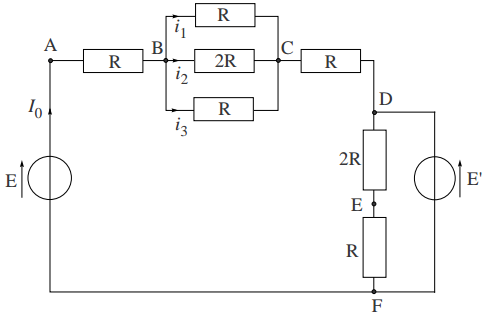
\includegraphics[width=\textwidth]{images/el7.png}
\end{minipage}
\end{boiteexercice}

\begin{boitecorrige}
\textbf{1.} La branche $\{D,\,2R,\,R,\,F\}$ constitue un diviseur de tension soumis à $E'$ :
\[
\boxed{U_{EF} = \frac{R}{R + 2R}\,E' = \frac{1}{3}\times3 = \qty{1}{V}}
\]

\textbf{2.} La résistance équivalente entre B et C est :
\[
R_{eq} = (R \parallel R) \parallel 2R = \frac{R}{2} \parallel 2R = \frac{\frac{R}{2}\times 2R}{\frac{R}{2}+2R} = \frac{R^2}{\frac{5R}{2}} = \frac{2R}{5}
\]
La branche $\{D, 2R, R, F\}$ est en parallèle avec $E'$ qui impose la tension à ses bornes. Du point de vue de la branche principale, les deux f.é.m. $E$ et $E'$ s'opposent (en série, sens contraires) ; la f.é.m. résultante est $E_0 = E - E' = \qty{2}{V}$.

La résistance totale de la maille principale est $R_0 = R + R_{eq} + R = R + \frac{2R}{5} + R = \frac{12R}{5} = \frac{12}{5}\,\Omega$.
\[
\boxed{I_0 = \frac{E_0}{R_0} = \frac{E-E'}{R_0} = \frac{2}{\frac{12}{5}} = \frac{5}{6}\,\text{A} \approx \qty{0.83}{A}}
\]

\textbf{3.} Le courant $I''$ circulant de D vers F dans la branche contenant $3R$ (soumise à $E'$) est, en convention récepteur :
\[
I'' = \frac{E'}{3R} = \frac{3}{3\times1} = \qty{1}{A}
\]
En définissant $I'$ en convention générateur par rapport à $E'$ (sens F $\to$ D dans $E'$), la loi des n\oe{}uds en D donne :
\[
\boxed{I' = I'' - I_0 = 1 - \frac{5}{6} = \frac{1}{6}\,\text{A} \approx \qty{0.17}{A} \quad (\text{de F vers D})}
\]

\textbf{4.} Par symétrie du réseau entre B et C : $i_1 = i_3$. Diviseur de courant en B :
\[
\boxed{i_1 = i_3 = \frac{R_{eq}}{R}\,I_0 = \frac{2R/5}{R}\,I_0 = \frac{2}{5}\times\frac{5}{6} = \frac{1}{3}\,\text{A} \approx \qty{0.33}{A}}
\]
\[
\boxed{i_2 = \frac{R_{eq}}{2R}\,I_0 = \frac{2R/5}{2R}\,I_0 = \frac{1}{5}\times\frac{5}{6} = \frac{1}{6}\,\text{A} \approx \qty{0.17}{A}}
\]
Vérification : $I_0 = i_1 + i_2 + i_3 = \frac{1}{3}+\frac{1}{6}+\frac{1}{3} = \frac{5}{6}$. Correct.
\end{boitecorrige}

\begin{center}
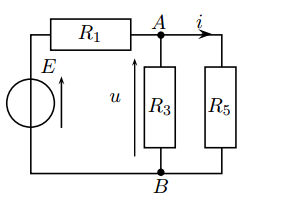
\includegraphics[width=0.5\textwidth]{images/electrocinetique/elec-002-006.png}
\captionof{figure}{\small Circuit linéaire : schéma avec sources et résistances.}
\end{center}
\begin{center}

\includegraphics[width=0.5\textwidth]{images/electrocinetique/elec-002-007.png}
\captionof{figure}{\small Analyse du circuit par les lois de Kirchhoff.}
\end{center}

\subsection*{Exercice 3 - Théorème de Thévenin \niveau{\moyen}}

\begin{boiteexercice}
\begin{center}
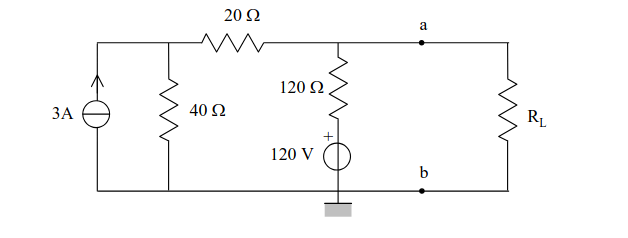
\includegraphics[width=0.7\textwidth]{images/el20.png}
\end{center}
$R_L$ est la résistance de charge.
\begin{enumerate}
  \item Déterminer le circuit équivalent de Thévenin vu entre les points a et b.
  \item Quelle valeur de $R_L$ permet de transmettre la puissance maximale à la charge ? Calculer cette puissance.
  \item Calculer la puissance transmise si $R_L = 2R_{th}$.
\end{enumerate}
\end{boiteexercice}

\begin{boitecorrige}
\textbf{1.} Par le calcul (tensions à vide et court-circuit) :
\[
E_{th} = \qty{120}{V} \qquad R_{th} = \qtyohm{40}
\]

\textbf{2.} La condition d'adaptation d'impédance donne la puissance maximale pour $R_L = R_{th}$ :
\[
\boxed{R_L = R_{th} = \qtyohm{40}}
\]
\[
P_{\max} = R_L\left(\frac{E_{th}}{R_L + R_{th}}\right)^2 = 40\times\left(\frac{120}{80}\right)^2 = 40\times2{,}25 = \qty{90}{W}
\]

\textbf{3.} Pour $R_L = 2R_{th} = \qtyohm{80}$ :
\[
P = 80\times\left(\frac{120}{80+40}\right)^2 = 80\times\left(\frac{120}{120}\right)^2 = 80\times1 = \qty{80}{W}
\]
\end{boitecorrige}

\subsection*{Exercice 4 - Théorème de Millman \niveau{\moyen}}

\begin{boiteexercice}
\begin{center}
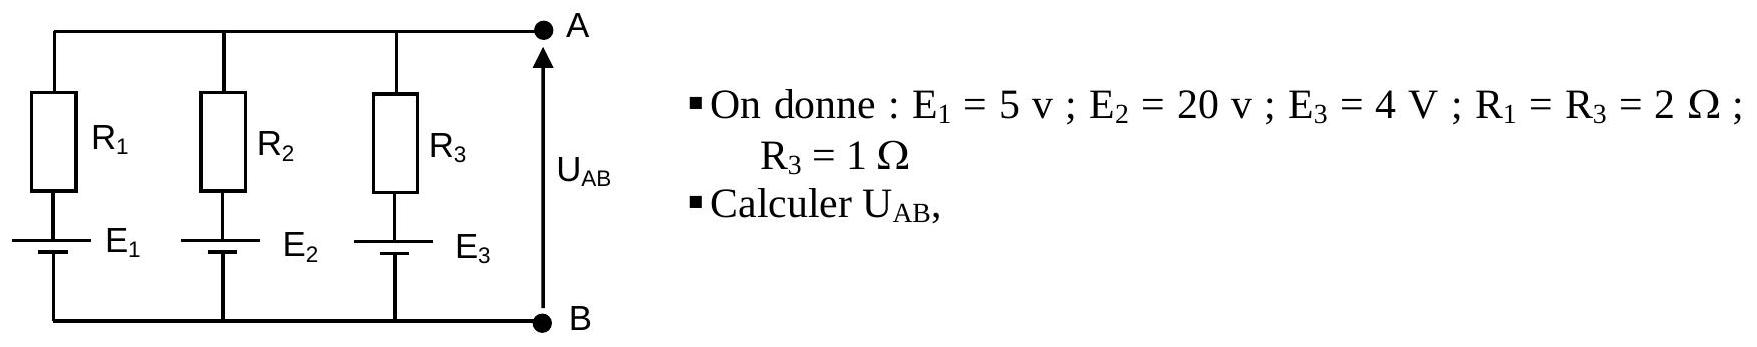
\includegraphics[width=0.85\textwidth]{images/el23.png}
\end{center}
\begin{enumerate}
  \item Calculer $U_{AB}$ en utilisant le théorème de Millman.
  \item Déterminer le courant $I$ traversant $R_4$.
\end{enumerate}
\end{boiteexercice}

\begin{boitecorrige}
\textbf{1.} On applique le théorème de Millman entre les n\oe{}uds A et B. Les trois branches en parallèle contiennent respectivement les f.é.m. $E_1 = \qty{4}{V}$ (sens B$\to$A), $E_2 = \qty{5}{V}$ (sens A$\to$B), $E_3 = \qty{8}{V}$ (sens B$\to$A), avec $R_1 = \qtyohm{2}$, $R_2 = \qtyohm{1}$, $R_3 = \qtyohm{2}$ :
\[
U_{AB} = \frac{-\dfrac{E_1}{R_1}+\dfrac{E_2}{R_2}-\dfrac{E_3}{R_3}}{\dfrac{1}{R_1}+\dfrac{1}{R_2}+\dfrac{1}{R_3}} = \frac{-\dfrac{4}{2}+\dfrac{5}{1}-\dfrac{8}{2}}{\dfrac{1}{2}+\dfrac{1}{1}+\dfrac{1}{2}} = \frac{-2+5-4}{0{,}5+1+0{,}5} = \frac{-1}{2} = \qty{-0.5}{V}
\]

\begin{boiteremarque}
Le signe de chaque f.é.m. dans Millman dépend de son sens par rapport au sens de référence A$\to$B. Une f.é.m. qui pousse dans le sens A$\to$B est positive, dans le sens B$\to$A est négative.
\end{boiteremarque}

\textbf{2.} Par l'équivalent de Thévenin avec $E_{th} = U_{AB}$ et $R_{th} = R_1\parallel R_2\parallel R_3 = \qtyohm{0.5}$ :
\[
I = \frac{E_{th}}{R_{th}+R_4} = \frac{0{,}5}{0{,}5 + R_4}
\]
(voir figure el24.png pour la valeur numérique de $R_4$).
\end{boitecorrige}

\begin{center}
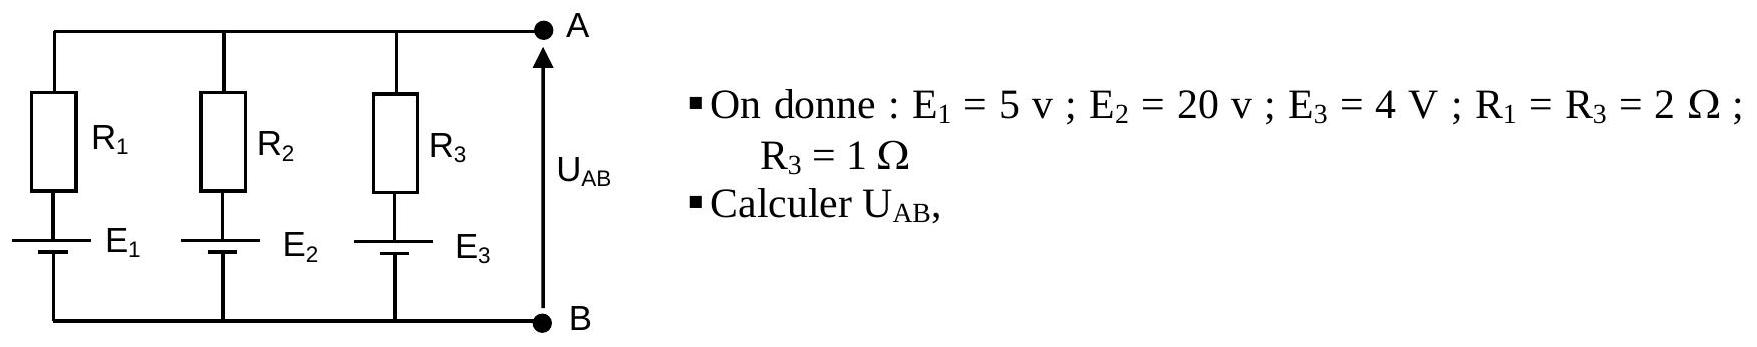
\includegraphics[width=0.7\textwidth]{images/electrocinetique/elec-004-014.png}
\captionof{figure}{\small Théorème de Millman : application à un n\oe{}ud à plusieurs branches.}
\end{center}

\subsection*{Exercice 5 - Théorème de Norton \niveau{\facile}}

\begin{boiteexercice}
Déterminer les modèles équivalents de Norton des circuits placés à gauche de AB dans chacun des schémas suivants.

\begin{minipage}{0.48\textwidth}
\centering
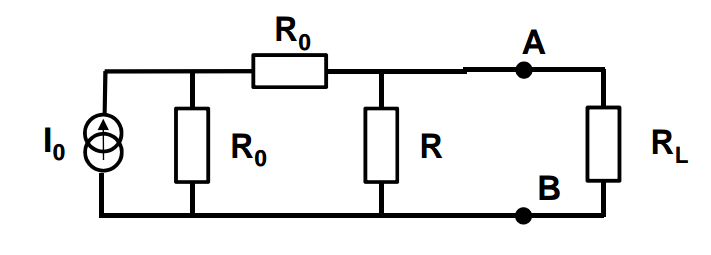
\includegraphics[width=\textwidth]{images/el31.png}
\end{minipage}
\hfill
\begin{minipage}{0.48\textwidth}
\centering
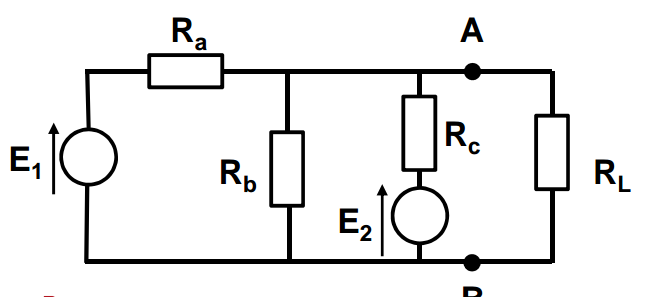
\includegraphics[width=\textwidth]{images/el32.png}
\end{minipage}
\end{boiteexercice}

\begin{boitecorrige}
\textbf{Schéma 1 :} Le courant de court-circuit $I_{AB}$ (obtenu en court-circuitant A et B) est la moitié du courant source : $I_{AB} = I_0/2$. La résistance équivalente (source de courant éteinte, c.-à-d. ouverte) est $R_{AB} = R \parallel 2R_0$.

\textbf{Schéma 2 :} Le courant de court-circuit (source de tension $E_1$ en série avec $R_a$, bornes AB court-circuitées) donne $I_{AB} = E_1/R_a$. La résistance équivalente (source $E_1$ éteinte) : $R_{AB} = R_a \parallel R_b \parallel R_c$.
\end{boitecorrige}

\begin{center}
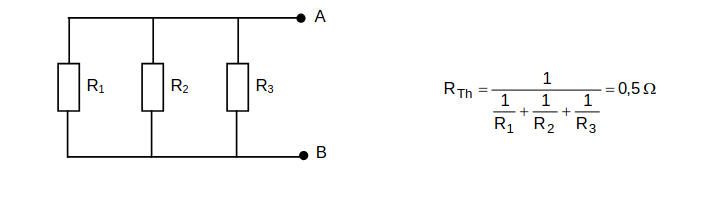
\includegraphics[width=0.6\textwidth]{images/electrocinetique/elec-005-015.png}
\captionof{figure}{\small Modèle équivalent de Norton : source de courant en parallèle avec une résistance.}
\end{center}
\begin{center}

\includegraphics[width=0.6\textwidth]{images/electrocinetique/elec-005-016.png}
\captionof{figure}{\small Transformation Norton $\leftrightarrow$ Thévenin : équivalence des modèles.}
\end{center}
\begin{center}
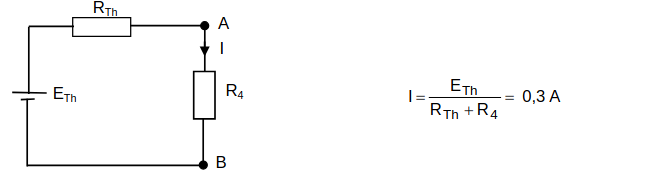
\includegraphics[width=0.6\textwidth]{images/electrocinetique/elec-005-017.png}
\captionof{figure}{\small Calcul du courant de court-circuit $I_{AB}$ pour le schéma 1.}
\end{center}
\begin{center}

\includegraphics[width=0.6\textwidth]{images/electrocinetique/elec-005-018.png}
\captionof{figure}{\small Calcul de la résistance équivalente $R_{AB}$ pour le schéma 2.}
\end{center}

\subsection*{Exercice 6 - Circuits en régime sinusoïdal \niveau{\difficile}}

\begin{boiteexercice}
\begin{center}
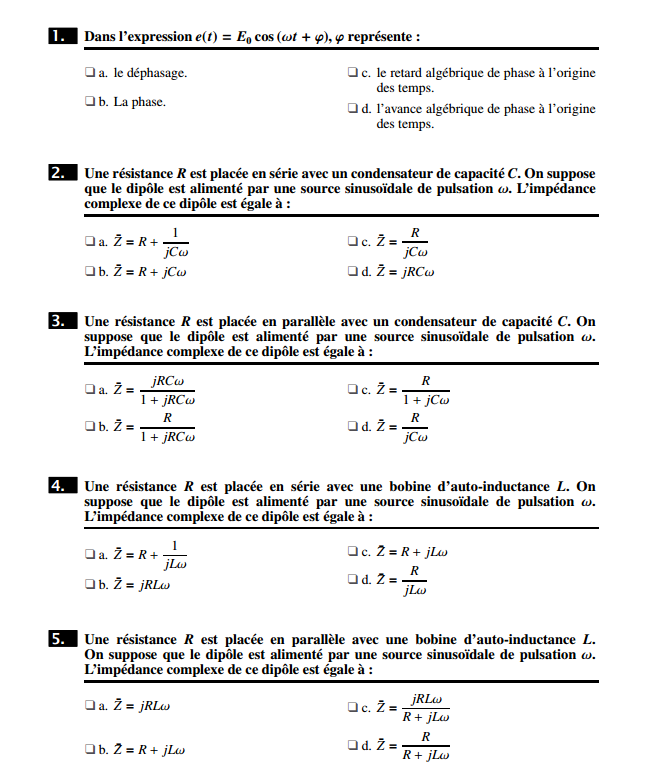
\includegraphics[width=0.65\textwidth]{images/el27.png}
\end{center}
\begin{center}
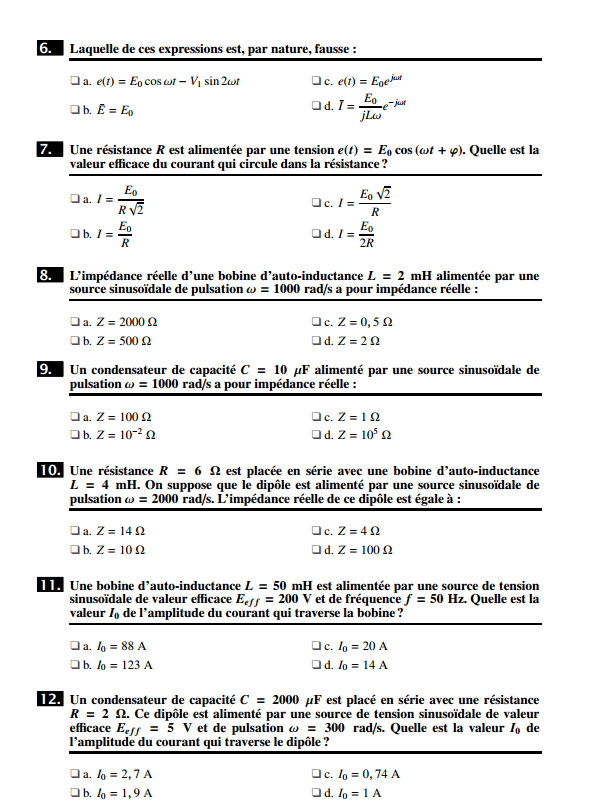
\includegraphics[width=0.65\textwidth]{images/el28.png}
\end{center}
Répondre aux questions posées sur les figures.
\end{boiteexercice}

\clearpage
\begin{boitecorrige}
\begin{center}
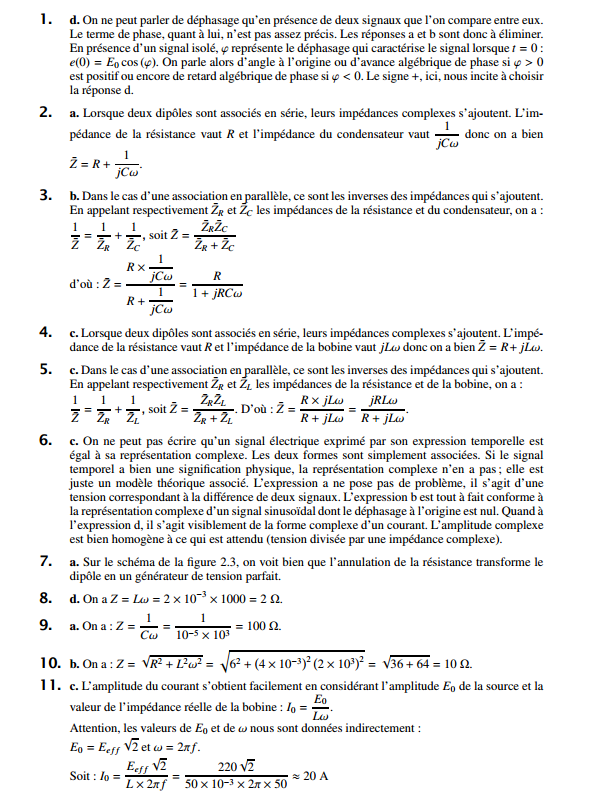
\includegraphics[width=0.7\textwidth]{images/el29.png}
\end{center}
\begin{center}
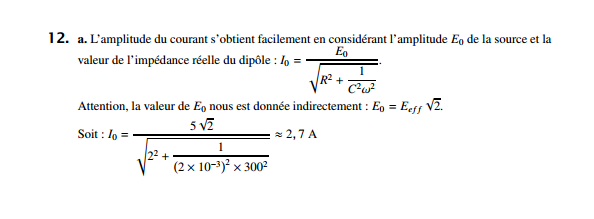
\includegraphics[width=0.7\textwidth]{images/el30.png}
\end{center}
\end{boitecorrige}

\begin{center}
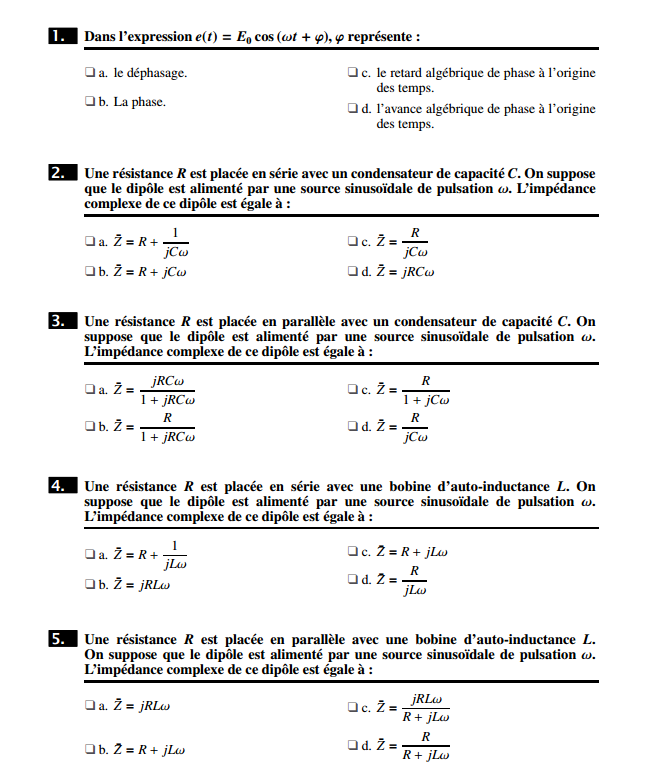
\includegraphics[height=0.5\textheight]{images/electrocinetique/elec-006-023.png}
\captionof{figure}{\small Circuit en régime sinusoïdal : représentation complexe des impédances.}
\end{center}
\begin{center}

\includegraphics[height=0.5\textheight]{images/electrocinetique/elec-006-024.png}
\captionof{figure}{\small Diagramme de Fresnel des tensions et courants en régime sinusoïdal.}
\end{center}

\section{Régimes transitoires}

\subsection*{Exercice 7 - Circuit RC : charge et décharge \niveau{\moyen}}

\begin{boiteexercice}
\begin{center}
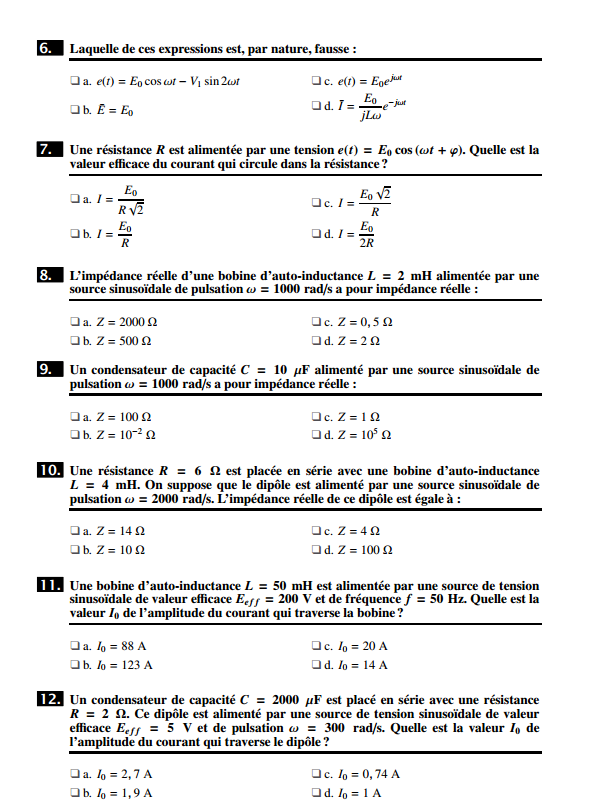
\includegraphics[height=0.45\textheight]{images/electrocinetique/elec-007-025.png}
\captionof{figure}{\small Circuit RC : charge et décharge d'un condensateur à travers une résistance.}
\end{center}
Un condensateur $C = \qty{10}{\mu F}$ est initialement déchargé. On le charge à travers $R = \qty{100}{k\Omega}$ par un générateur de f.é.m. $E = \qty{12}{V}$.
\begin{enumerate}
  \item Écrire l'équation différentielle régissant la tension $u_C(t)$ aux bornes du condensateur.
  \item Résoudre et tracer qualitativement $u_C(t)$.
  \item Calculer la constante de temps $\tau$ et le temps pour atteindre $95\,\%$ de la charge finale.
  \item On ouvre le circuit quand $u_C = \qty{8}{V}$. La résistance de décharge est $R' = \qty{50}{k\Omega}$. Écrire et résoudre l'équation de décharge.
\end{enumerate}
\end{boiteexercice}

\begin{boitecorrige}
\textbf{1.} La loi des mailles donne : $E = Ri + u_C$ avec $i = C\,\d u_C/\d t$ :
\[
RC\,\frac{\d u_C}{\d t} + u_C = E
\]

\textbf{2.} L'équation homogène $RC\,\d u_C/\d t + u_C = 0$ a pour solution $u_C^{hom} = Ke^{-t/\tau}$ avec $\tau = RC$. Solution particulière $u_C^{part} = E$.
\[
u_C(t) = E(1-e^{-t/\tau}) \quad \text{avec } u_C(0)=0
\]

\textbf{3.} $\tau = RC = 10^5\times10^{-5} = \qty{1}{s}$.

$u_C(t_{95}) = 0{,}95E$ donne $1-e^{-t_{95}/\tau}=0{,}95$, soit $e^{-t_{95}}=0{,}05$, $t_{95} = -\ln(0{,}05) \approx 3\tau = \qty{3}{s}$.

\textbf{4.} La décharge part de $u_0=\qty{8}{V}$ avec constante $\tau' = R'C = 5\times10^4\times10^{-5} = \qty{0.5}{s}$ :
\[
u_C(t) = u_0\,e^{-t/\tau'} = 8e^{-2t} \quad [\text{V}], \quad t\geq0
\]
(l'origine du temps est remise à zéro au moment de l'ouverture).
\end{boitecorrige}

\subsection*{Exercice 8 - Circuit RL en régime transitoire \niveau{\moyen}}

\begin{boiteexercice}
\begin{center}
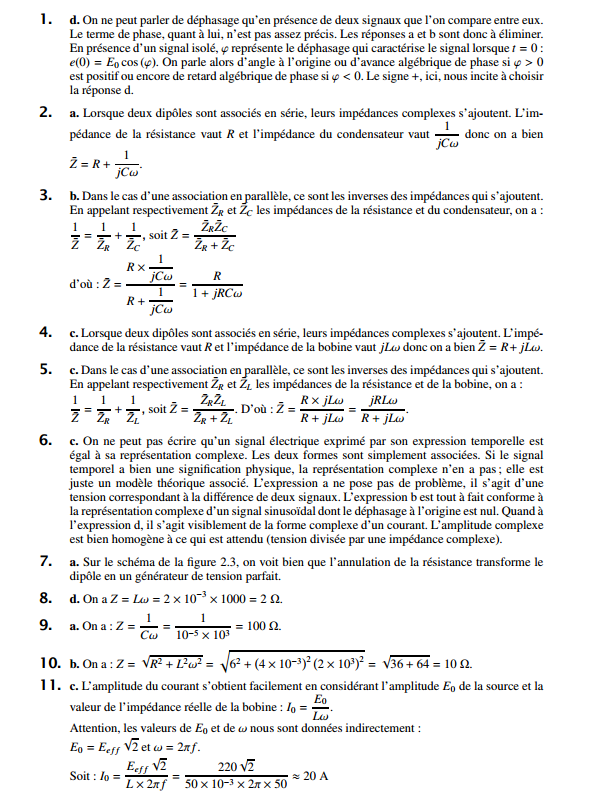
\includegraphics[height=0.45\textheight]{images/electrocinetique/elec-008-027.png}
\captionof{figure}{\small Circuit RL : établissement et rupture du courant dans une bobine.}
\end{center}
Un circuit RL série comporte $R = \qty{50}{\Omega}$ et $L = \qty{100}{mH}$. À $t=0$, on connecte une source de tension $E = \qty{10}{V}$.
\begin{enumerate}
  \item Écrire l'équation différentielle du courant $i(t)$.
  \item Trouver $i(t)$ sachant que $i(0) = 0$.
  \item Calculer $\tau$, $i_{max}$ et le courant à $t=\tau$.
  \item Calculer l'énergie stockée dans l'inductance en régime permanent.
\end{enumerate}
\end{boiteexercice}

\begin{boitecorrige}
\textbf{1.} Loi des mailles :
\[
L\frac{\d i}{\d t}+Ri = E
\]

\textbf{2.} Séparation homogène + particulière :
\[
i(t) = \frac{E}{R}\left(1-e^{-t/\tau}\right) \quad \text{avec}\quad \tau=\frac{L}{R}
\]

\textbf{3.} $\tau = L/R = 0{,}1/50 = \qty{2}{ms}$. $i_{max} = E/R = 10/50 = \qty{200}{mA}$.
$i(\tau) = i_{max}(1-e^{-1}) = 0{,}2\times(1-0{,}368) \approx \qty{126}{mA} \approx 63{,}2\,\%$ de $i_{max}$.

\textbf{4.} En régime permanent, $i = i_{max} = \qty{200}{mA}$ :
\[
W_L = \frac{1}{2}Li_{max}^2 = \frac{1}{2}\times0{,}1\times(0{,}2)^2 = \qty{2}{mJ}
\]
\end{boitecorrige}

\section{Régime sinusoïdal forcé}

\subsection*{Exercice 9 - Impédance complexe \niveau{\moyen}}

\begin{boiteexercice}
Un circuit RLC série est alimenté par $e(t) = E_0\cos(\omega t)$ avec $E_0 = \qty{10}{V}$, $R = \qty{10}{\Omega}$, $L = \qty{100}{mH}$, $C = \qty{100}{\mu F}$, $\omega = \qty{200}{rad.s^{-1}}$.
\begin{enumerate}
  \item Calculer les impédances $Z_R$, $Z_L$, $Z_C$ et l'impédance totale $Z$.
  \item Calculer l'intensité maximale $I_0$ et le déphasage $\varphi$ entre la tension et le courant.
  \item Calculer les tensions efficaces aux bornes de chaque élément.
  \item Exprimer $i(t)$ et $u_R(t)$.
\end{enumerate}
\end{boiteexercice}

\begin{boitecorrige}
\textbf{1.} $Z_R = R = \qty{10}{\Omega}$, $Z_L = j\omega L = j\times200\times0{,}1 = j\qty{20}{\Omega}$, $Z_C = \frac{1}{j\omega C} = \frac{1}{j\times200\times10^{-4}} = \frac{-j}{0{,}02} = -j\qty{50}{\Omega}$.
\[
Z = R+j\omega L+\frac{1}{j\omega C} = 10+j20-j50 = 10-j30 = \sqrt{10^2+30^2}\,\angle\arctan(-30/10)
\]
\[
|Z| = \sqrt{100+900} = \sqrt{1000} \approx \qty{31.6}{\Omega}, \quad \varphi = \arctan(-3) \approx -71{,}6^\circ 
\]

\textbf{2.} $I_0 = E_0/|Z| = 10/31{,}6 \approx \qty{316}{mA}$. Le déphasage $\varphi\approx-71{,}6^\circ $ : le courant est en avance sur la tension (circuit capacitif).

\textbf{3.} Valeurs efficaces : $U_R = RI_{eff} = 10\times0{,}316/\sqrt{2} \approx \qty{2.24}{V}$, $U_L = \omega L\cdot I_{eff} = 20\times\qty{0.224}{A} \approx \qty{4.47}{V}$, $U_C = I_{eff}/(\omega C) = 50\times\qty{0.224}{A} \approx \qty{11.2}{V}$.

\textbf{4.}
\[
i(t) = I_0\cos(\omega t-\varphi) = 0{,}316\cos(200t+71{,}6^\circ ) \quad [\text{A}]
\]
\[
u_R(t) = Ri(t) = 3{,}16\cos(200t+71{,}6^\circ ) \quad [\text{V}]
\]
\end{boitecorrige}

\subsection*{Exercice 10 - Résonance en série \niveau{\difficile}}

\begin{boiteexercice}
Reprendre le circuit RLC série de l'exercice précédent.
\begin{enumerate}
  \item À quelle pulsation $\omega_0$ se produit la résonance ? Calculer $\omega_0$.
  \item Quelle est la valeur maximale du courant à la résonance ?
  \item Définir et calculer le facteur de qualité $Q$.
  \item La bande passante $\Delta\omega$ est définie par les pulsations $\omega_\pm$ pour lesquelles $I = I_{max}/\sqrt{2}$. Calculer $\Delta\omega$.
\end{enumerate}
\end{boiteexercice}

\begin{boitecorrige}
\textbf{1.} La résonance se produit quand $\text{Im}(Z) = 0$, soit $\omega L = 1/(\omega C)$ :
\[
\omega_0 = \frac{1}{\sqrt{LC}} = \frac{1}{\sqrt{0{,}1\times10^{-4}}} = \frac{1}{\sqrt{10^{-5}}} = \frac{1}{10^{-5/2}} = 10^{5/2} \approx \qty{316}{rad.s^{-1}}
\]

\textbf{2.} À la résonance, $Z = R$ (l'inductance et le condensateur se compensent) :
\[
I_{max} = \frac{E_0}{R} = \frac{10}{10} = \qty{1}{A}
\]

\textbf{3.} Le facteur de qualité :
\[
Q = \frac{\omega_0 L}{R} = \frac{316\times0{,}1}{10} = \qty{3.16}{}
\]
Ou encore $Q = 1/(\omega_0 CR) = 1/(316\times10^{-4}\times10) \approx 3{,}16$.

\textbf{4.} La bande passante est $\Delta\omega = \omega_0/Q = 316/3{,}16 = \qty{100}{rad.s^{-1}}$.

Les pulsations de coupure à $-3\,\text{dB}$ : $\omega_\pm = \omega_0\pm\Delta\omega/2 = 316\pm50$, soit $\omega_+ = \qty{366}{rad.s^{-1}}$ et $\omega_- = \qty{266}{rad.s^{-1}}$.
\end{boitecorrige}

\subsection*{Exercice 11 - Filtres du premier ordre \niveau{\moyen}}

\begin{boiteexercice}
\begin{enumerate}
  \item On considère un filtre RC (résistance en série, condensateur en sortie). Montrer que la fonction de transfert est $H(j\omega) = \frac{1}{1+j\omega RC}$ et que c'est un filtre passe-bas.
  \item Calculer la fréquence de coupure $f_c$ pour $R = \qty{1}{k\Omega}$ et $C = \qty{1}{\mu F}$.
  \item Calculer le gain en dB et le déphasage à $f = f_c$, $f = f_c/10$ et $f = 10f_c$.
  \item Si on inverse $R$ et $C$ (condensateur en série, résistance en sortie), montrer que c'est un filtre passe-haut.
\end{enumerate}
\end{boiteexercice}

\begin{boitecorrige}
\textbf{1.} Par le diviseur de tension : $U_s = \frac{Z_C}{Z_R+Z_C}U_e = \frac{1/(j\omega C)}{R+1/(j\omega C)}U_e$.
\[
H(j\omega) = \frac{U_s}{U_e} = \frac{1}{1+j\omega RC}
\]
$|H| = 1/\sqrt{1+(\omega RC)^2}$ est une fonction décroissante de $\omega$ : c'est bien un \textbf{filtre passe-bas}.

\textbf{2.} La fréquence de coupure est définie par $|H(j\omega_c)| = 1/\sqrt{2}$ :
\[
\omega_c = \frac{1}{RC} = \frac{1}{10^3\times10^{-6}} = \qty{1000}{rad.s^{-1}}, \quad f_c = \frac{\omega_c}{2\pi} \approx \qty{159}{Hz}
\]

\textbf{3.}
\begin{center}
\begin{tabular}{lccc}
\toprule
$f$ & $|H|$ & Gain (dB) & $\varphi = -\arctan(\omega RC)$\\
\midrule
$f_c/10$ & $\approx1$ & $\approx0\,\text{dB}$ & $\approx -5{,}7^\circ $\\
$f_c$ & $1/\sqrt{2}$ & $-3\,\text{dB}$ & $-45^\circ $\\
$10f_c$ & $\approx0{,}1$ & $\approx-20\,\text{dB}$ & $\approx -84^\circ $\\
\bottomrule
\end{tabular}
\end{center}
Au-delà de $f_c$, le gain diminue de $-20\,\text{dB/décade}$ (pente du diagramme de Bode asymptotique).

\textbf{4.} En intervertissant : $U_s = \frac{R}{R+1/(j\omega C)}U_e = \frac{j\omega RC}{1+j\omega RC}U_e$.
$|H| = \omega RC/\sqrt{1+(\omega RC)^2}$ est croissante avec $\omega$ : \textbf{filtre passe-haut}.
\end{boitecorrige}

\subsection*{Exercice 12 - Puissance en régime sinusoïdal \niveau{\moyen}}

\begin{boiteexercice}
Un circuit RL est alimenté par une tension sinusoïdale $u(t) = 230\sqrt{2}\cos(100\pi t)$ V, avec $R=\qty{30}{\Omega}$ et $L = \qty{0.1}{H}$.
\begin{enumerate}
  \item Calculer l'impédance, le courant efficace et le déphasage.
  \item Calculer la puissance active $P$, la puissance réactive $Q$ et la puissance apparente $S$.
  \item Calculer le facteur de puissance $\cos\varphi$.
  \item Pour relever le facteur de puissance à $0{,}99$, quelle capacité $C$ faut-il mettre en parallèle ?
\end{enumerate}
\end{boiteexercice}

\begin{boitecorrige}
\textbf{1.} $\omega = 100\pi \approx \qty{314}{rad.s^{-1}}$.
$|Z| = \sqrt{R^2+(\omega L)^2} = \sqrt{900+(31{,}4)^2} = \sqrt{900+986} = \sqrt{1886} \approx \qty{43.4}{\Omega}$.
$I_{eff} = U_{eff}/|Z| = 230/43{,}4 \approx \qty{5.30}{A}$.
$\varphi = \arctan(\omega L/R) = \arctan(31{,}4/30) \approx \arctan(1{,}047) \approx 46{,}3^\circ $.

\textbf{2.} $P = U_{eff}I_{eff}\cos\varphi = 230\times5{,}30\times\cos(46{,}3^\circ ) \approx 230\times5{,}30\times0{,}692 \approx \qty{843}{W}$.
$Q = U_{eff}I_{eff}\sin\varphi \approx 230\times5{,}30\times0{,}721 \approx \qty{879}{VAR}$.
$S = U_{eff}I_{eff} = 230\times5{,}30 \approx \qty{1219}{VA}$.

\textbf{3.} $\cos\varphi = P/S = 843/1219 \approx 0{,}692$.

\textbf{4.} Pour $\cos\varphi'=0{,}99$, $\sin\varphi'=\sqrt{1-0{,}99^2}\approx0{,}141$. La puissance réactive à compenser :
$Q' = P\tan\varphi'= 843\times(0{,}141/0{,}99)\approx \qty{120}{VAR}$.
La capacité en parallèle doit fournir $Q_C = Q-Q' = 879-120 = \qty{759}{VAR} = U_{eff}^2\omega C$.
\[
C = \frac{Q_C}{U_{eff}^2\omega} = \frac{759}{230^2\times314} \approx \qty{45.6}{\mu F}
\]
\end{boitecorrige}


\subsection*{Exercice 13 - Régime transitoire RC : charge et décharge \niveau{\moyen}}

\begin{boiteexercice}
Un circuit RC série est composé d'une résistance $R=\qty{10}{k\Omega}$ et d'un condensateur $C=\qty{100}{\mu F}$. À $t=0$, on applique une tension continue $E=\qty{12}{V}$ (condensateur initialement déchargé).
\begin{enumerate}
  \item Écrire l'équation différentielle régissant $V_C(t)$.
  \item Donner la solution $V_C(t)$ en phase de charge. Calculer la constante de temps $\tau$ et le temps à mi-charge $t_{1/2}$.
  \item Calculer $V_C$ et $i$ à $t=\tau$, $t=2\tau$, $t=5\tau$.
  \item Le condensateur, chargé à $E=12\;\text{V}$, se décharge dans la même résistance $R$. Donner $V_C(t)$ et $i(t)$ en décharge.
  \item Calculer l'énergie stockée dans le condensateur et l'énergie dissipée dans $R$ pendant la charge complète.
\end{enumerate}
\end{boiteexercice}

\begin{boitecorrige}
\textbf{1.} La loi des mailles donne $E = Ri(t) + V_C(t)$ avec $i=C\,\dot V_C$ :
\[
RC\,\dot V_C + V_C = E \implies \tau\dot V_C + V_C = E, \quad \tau = RC
\]

\textbf{2.} Solution avec C.I. $V_C(0)=0$ :
\[
\boxed{V_C(t) = E\!\left(1-\e^{-t/\tau}\right)}
\]
\[
\tau = RC = 10\times10^3\times100\times10^{-6} = \qty{1}{s}
\]
Temps à mi-charge ($V_C = E/2$) :
\[
\frac{1}{2} = 1-\e^{-t_{1/2}/\tau} \implies \e^{-t_{1/2}} = \frac{1}{2} \implies t_{1/2} = \tau\ln 2 \approx \qty{0.693}{s}
\]

\textbf{3.} Courant $i(t) = (E/R)\e^{-t/\tau}$, $I_0 = E/R = 12/10000 = \qty{1.2}{mA}$.
\begin{center}
\begin{tabular}{c|c|c}
$t$ & $V_C$ (V) & $i$ (mA)\\
\hline
$\tau=1\;\text{s}$ & $12(1-1/e)=7{,}58$ & $1{,}2/e=0{,}441$\\
$2\tau$ & $12(1-e^{-2})=10{,}38$ & $1{,}2e^{-2}=0{,}162$\\
$5\tau$ & $12(1-e^{-5})=11{,}92$ & $1{,}2e^{-5}=0{,}008$\\
\end{tabular}
\end{center}
À $t=5\tau$, le condensateur est chargé à $\approx99{,}3\;\%$ de sa valeur finale.

\textbf{4.} Lors de la décharge ($V_C(0)=E$, source déconnectée) :
\[
V_C(t) = E\,\e^{-t/\tau} = 12\e^{-t}\;\text{V}, \qquad i(t) = -\frac{E}{R}\e^{-t/\tau} = -1{,}2\e^{-t}\;\text{mA}
\]
(le signe négatif indique que le courant circule en sens opposé à la charge).

\textbf{5.} Énergie stockée : $E_C = \frac{1}{2}CE^2 = \frac{1}{2}\times100\times10^{-6}\times144 = \qty{7.2}{mJ}$.

L'énergie fournie par la source pendant la charge :
\[
E_\text{source} = \int_0^\infty E\,i(t)\,\mathrm{d}t = \frac{E^2}{R}\int_0^\infty\e^{-t/\tau}\mathrm{d}t = \frac{E^2\tau}{R} = CE^2 = \qty{14.4}{mJ}.
\]

L'énergie dissipée dans $R$ : $E_R = E_\text{source} - E_C = 14{,}4 - 7{,}2 = \qty{7.2}{mJ}$. On note que $E_R = E_C$ : quel que soit $R$, exactement la moitié de l'énergie fournie est dissipée dans la résistance.
\end{boitecorrige}

\subsection*{Exercice 14 - Filtre RC passe-bas \niveau{\moyen}}

\begin{boiteexercice}
Un filtre passe-bas RC est formé d'une résistance $R=\qty{1}{k\Omega}$ en série avec un condensateur $C=\qty{0.1}{\mu F}$. La tension d'entrée est $u_e(t) = U_0\cos(\omega t)$ et la tension de sortie est prise aux bornes de $C$.
\begin{enumerate}
  \item Exprimer la fonction de transfert $\underline{H}(j\omega) = \underline{U}_s/\underline{U}_e$ en notation complexe.
  \item Calculer le module $|\underline{H}|$ et la phase $\varphi = \arg(\underline{H})$.
  \item Calculer la fréquence de coupure $f_c$ et vérifier que $|\underline{H}(j\omega_c)| = 1/\sqrt{2}$.
  \item Tracer qualitativement le diagramme de Bode (gain en dB et phase) en identifiant les asymptotes.
  \item Pour $f=f_c/10$, $f=f_c$ et $f=10f_c$, calculer $|\underline{H}|$ et $\varphi$.
\end{enumerate}
\end{boiteexercice}

\begin{boitecorrige}
\textbf{1.} Le diviseur de tension complexe donne :
\[
\underline{H}(j\omega) = \frac{Z_C}{Z_R+Z_C} = \frac{1/(j\omega C)}{R+1/(j\omega C)} = \frac{1}{1+j\omega RC} = \frac{1}{1+j\omega\tau}
\]
avec $\tau = RC$.

\textbf{2.} Module et phase :
\[
|\underline{H}| = \frac{1}{\sqrt{1+(\omega\tau)^2}}, \qquad \varphi = -\arctan(\omega\tau)
\]

\textbf{3.} $\tau = RC = 10^3\times10^{-7} = 10^{-4}\;\text{s}$.
\[
f_c = \frac{1}{2\pi\tau} = \frac{1}{2\pi\times10^{-4}} \approx \qty{1592}{Hz} \approx \qty{1.59}{kHz}
\]
Vérification : à $\omega=\omega_c=1/\tau$, $|\underline{H}| = 1/\sqrt{1+1} = 1/\sqrt{2}$.

\textbf{4.} Diagramme de Bode :
\begin{itemize}[nosep]
  \item Gain $G_{dB} = 20\log|\underline{H}|$. Pour $\omega\ll\omega_c$ : $G_{dB}\to 0\;\text{dB}$ (asymptote horizontale). Pour $\omega\gg\omega_c$ : $G_{dB}\approx -20\log(\omega\tau)$ (pente $-20\;\text{dB/décade}$). Au coude : $G_{dB}(f_c) = -3\;\text{dB}$.
  \item Phase : de $0^\circ $ à $-90^\circ $, avec $\varphi(f_c) = -45^\circ $.
\end{itemize}

\textbf{5.} Valeurs numériques :
\begin{center}
\renewcommand{\arraystretch}{1.2}
\begin{tabular}{|c|c|c|c|}
\hline
$f$ & $\omega\tau$ & $|\underline{H}|$ & $\varphi$\\
\hline
$f_c/10$ & $0{,}1$ & $1/\sqrt{1{,}01}\approx 0{,}995$ & $-5{,}7^\circ$\\
$f_c$ & $1$ & $1/\sqrt{2}\approx 0{,}707$ & $-45^\circ$\\
$10f_c$ & $10$ & $1/\sqrt{101}\approx 0{,}0995$ & $-84{,}3^\circ$\\
\hline
\end{tabular}
\end{center}
\end{boitecorrige}

\subsection*{Exercice 15 - Circuit RLC série résonant \niveau{\difficile}}

\begin{boiteexercice}
Un circuit RLC série comporte $R=\qty{50}{\Omega}$, $L=\qty{0.2}{H}$, $C=\qty{2}{\mu F}$, alimenté par $e(t) = E_0\cos(\omega t)$ avec $E_0=\qty{10}{V}$.
\begin{enumerate}
  \item Calculer la pulsation de résonance $\omega_0$ et la fréquence $f_0$.
  \item Calculer le facteur de qualité $Q$ et la bande passante $\Delta\omega$.
  \item Exprimer l'impédance $\underline{Z}(\omega)$ et montrer qu'à la résonance $|\underline{Z}|=R$.
  \item Calculer le courant efficace $I_0$ et les tensions efficaces $U_R$, $U_L$, $U_C$ à la résonance.
  \item À la résonance, comparer $U_L$ et $U_C$ à la tension source. Commenter (surtension).
\end{enumerate}
\end{boiteexercice}

\begin{boitecorrige}
\textbf{1.} Pulsation de résonance :
\[
\omega_0 = \frac{1}{\sqrt{LC}} = \frac{1}{\sqrt{0{,}2\times2\times10^{-6}}} = \frac{1}{\sqrt{4\times10^{-7}}} = \frac{1}{6{,}32\times10^{-4}} \approx \qty{1582}{rad/s}
\]
\[
f_0 = \frac{\omega_0}{2\pi} \approx \qty{252}{Hz}
\]

\textbf{2.} Facteur de qualité et bande passante :
\[
Q = \frac{\omega_0 L}{R} = \frac{1582\times0{,}2}{50} = \frac{316}{50} \approx 6{,}32
\]
\[
\Delta\omega = \frac{\omega_0}{Q} = \frac{1582}{6{,}32} \approx \qty{250}{rad/s}, \quad \Delta f = \frac{\Delta\omega}{2\pi} \approx \qty{39.8}{Hz}
\]

\textbf{3.} Impédance complexe :
\[
\underline{Z}(\omega) = R + j\omega L + \frac{1}{j\omega C} = R + j\!\left(\omega L - \frac{1}{\omega C}\right)
\]
À $\omega=\omega_0$ : $\omega_0 L = 1/(\omega_0 C)$ (car $\omega_0^2=1/LC$), donc la partie imaginaire s'annule et $|\underline{Z}(\omega_0)| = R$.

\textbf{4.} À la résonance, $I_0 = E_0/(\sqrt{2}R)$ (valeur efficace) :
\[
I_{\text{eff}} = \frac{E_0/\sqrt{2}}{R} = \frac{10/\sqrt{2}}{50} = \frac{10}{50\sqrt{2}} \approx \qty{141}{mA}
\]
\[
U_R = RI_\text{eff} = 50\times0{,}141 = \qty{7.07}{V}
\]
\[
U_L = \omega_0 L\,I_\text{eff} = 1582\times0{,}2\times0{,}141 = \qty{44.6}{V}
\]
\[
U_C = \frac{I_\text{eff}}{\omega_0 C} = \frac{0{,}141}{1582\times2\times10^{-6}} = \qty{44.6}{V}
\]

\textbf{5.} On constate que $U_L = U_C = Q\times U_\text{source,eff} = 6{,}32\times7{,}07 \approx \qty{44.6}{V} \gg U_\text{source,eff} = \qty{7.07}{V}$.
C'est le phénomène de \textbf{surtension de résonance} : les tensions aux bornes de $L$ et $C$ peuvent dépasser largement la tension d'alimentation d'un facteur $Q$. Ce phénomène est recherché dans les circuits accordés (radio) mais peut être dangereux dans d'autres applications.
\end{boitecorrige}

\subsection*{Exercice 16 - Loi de Faraday et transformateur idéal \niveau{\moyen}}

\begin{boiteexercice}
\textbf{Partie A -- Loi de Faraday.} Une spire circulaire de rayon $r=\qty{5}{cm}$ est plongée dans un champ magnétique $B(t)=B_0\cos(\omega t)$ avec $B_0=\qty{0.1}{T}$ et $f=\qty{50}{Hz}$, perpendiculaire au plan de la spire.
\begin{enumerate}
  \item Calculer le flux $\Phi(t)$ à travers la spire.
  \item Appliquer la loi de Faraday pour calculer la force électromotrice induite $e(t)$.
  \item Calculer la valeur maximale de $e$ et sa valeur efficace.
\end{enumerate}
\textbf{Partie B -- Transformateur idéal.} Un transformateur abaisseur a $N_1=2000$ spires au primaire et $N_2=200$ spires au secondaire. Le primaire est alimenté par $U_1=\qty{230}{V}$ efficaces.
\begin{enumerate}[resume]
  \item Calculer la tension secondaire $U_2$.
  \item Pour une charge $R_L=\qty{10}{\Omega}$ au secondaire, calculer $I_2$, $I_1$ et la puissance transmise.
  \item Vérifier que la conservation de l'énergie est assurée ($P_1=P_2$).
\end{enumerate}
\end{boiteexercice}

\begin{boitecorrige}
\textbf{Partie A.}

\textbf{1.} Flux à travers la spire :
\[
\Phi(t) = B(t)\cdot S = B_0\cos(\omega t)\cdot\pi r^2 = 0{,}1\times\pi\times(0{,}05)^2\cos(\omega t) = 7{,}85\times10^{-4}\cos(\omega t)\;\text{Wb}
\]

\textbf{2.} Loi de Faraday ($e = -\mathrm{d}\Phi/\mathrm{d}t$) :
\[
e(t) = -\frac{\mathrm{d}\Phi}{\mathrm{d}t} = B_0\pi r^2\omega\sin(\omega t) = \Phi_\text{max}\,\omega\sin(\omega t)
\]

\textbf{3.} Valeur maximale :
\[
e_\text{max} = B_0\pi r^2\omega = 7{,}85\times10^{-4}\times2\pi\times50 \approx \qty{0.247}{V}
\]
Valeur efficace : $E_\text{eff} = e_\text{max}/\sqrt{2} \approx \qty{0.175}{V}$.

\textbf{Partie B.}

\textbf{4.} Pour un transformateur idéal (pas de pertes) :
\[
\frac{U_2}{U_1} = \frac{N_2}{N_1} \implies U_2 = 230\times\frac{200}{2000} = \qty{23}{V}
\]

\textbf{5.} Courant secondaire :
\[
I_2 = \frac{U_2}{R_L} = \frac{23}{10} = \qty{2.3}{A}
\]
Courant primaire (conservation de la puissance instantanée, $I_1N_1=I_2N_2$) :
\[
I_1 = I_2\frac{N_2}{N_1} = 2{,}3\times\frac{200}{2000} = \qty{0.23}{A}
\]
Puissance transmise : $P = U_2 I_2 = 23\times2{,}3 = \qty{52.9}{W}$.

\textbf{6.} Puissance primaire : $P_1 = U_1 I_1 = 230\times0{,}23 = \qty{52.9}{W} = P_2$. L'énergie est bien conservée : le transformateur idéal ne dissipe aucune puissance.
\end{boitecorrige}

\ifdefined\inMainDoc\else\end{document}\fi
